%!TEX program = xelatex
\documentclass{xmu}
\usepackage{physics}
\usepackage{longtable}

%%%%%%%%%%%%%%%%%%%%%%%%%%%%%%%%%%%%%%%%%%%%%%%%%%%%%%%%%%
%%%%%%%%     XMU Undergraduates Thesis Template    %%%%%%%%
%%%%%%%%              Made by: F5Soft              %%%%%%%%
%%%%%%%%  https://github.com/F5Soft/xmu-template   %%%%%%%%
%%%%%%%%           Modified by: Astolfo            %%%%%%%%
%%%%%%%%  https://github.com/Astolfo/xmu-template  %%%%%%%%
%%%%%%%%%%%%%%%%%%%%%%%%%%%%%%%%%%%%%%%%%%%%%%%%%%%%%%%%%%

\begin{document}

% 电子版 / 打印版(取消注释下一行即为打印版)
\print
% 取消注释后,将在某些偶数页产生空白页,使得下一部分的内容从奇数页开始

% 取消注释后,仅使用数字作为章的编号
\arabicchapter

% 毕业设计 / 毕业论文(取消注释下一行即为毕业设计)
% \design

% 主修 / 辅修(取消注释下一行即为辅修, 这个别改)
\minor

% 标题
\title{中文标题}
{Title in English}
% 姓名
\author{}
% 学号
\idn{}
% 学院
\college{}
% 专业
\subject{}
% 年级
\grade{}
% 校内指导教师
\teacher{XXX\; 教授}
% 校外指导教师(注释则不显示, 按照要求是没有也得保留下面这种形式)
\otherteacher{(姓名)\; (职务)}

% 完成时间
\pubdate{}

% 关键词
\keywords{中文关键词}
{Keyword in English}

% 生成封面、承诺书
\maketitle

% 诚信承诺书
\vspace*{-2.45em}
\pagestyle{plain}
\begin{center}
    \sf\zihao{3}厦门大学本科学位论文诚信承诺书
\end{center}
\vspace{1.5em}
{
    \renewcommand{\baselinestretch}{2}
    \zihao{4}
    \par
    本人呈交的学位论文是在导师指导下独立完成的研究成果。本人在论文写作中参考其他个人或集体已经发表的研究成果,均在文中以适当方式 明确标明,并符合相关法律规范及《厦门大学本科毕业论文(设计)规范》。
    \par
    该学位论文为(XXX教授)课题(组)的研究成果,获得(XXX教授)课题(组)经费或实验室的资助,在(XXX教授)实验室完成(请在以上括号内填写课题或课题组负责人或实验室名称,未有此项声明内容的,可以不作特别声明)。
    \par
    本人承诺辅修专业毕业论文(设计)(如有)的内容与主修专业不存在相同与相近情况。
    \vspace{4em}
    \par
    \hfill 学生声明(签名):\qquad \qquad \qquad \quad~
    \par
    \hfill XXXX 年 XX 月 XX 日
    \par
}
\clearpage

\blankpagetitle

% 知悉书
\vspace*{-2.45em}
\pagestyle{plain}
\begin{center}
    \bf\songti\zihao{3}知\quad 悉\quad 书
\end{center}
\vspace{1.5em}
{
    \renewcommand{\baselinestretch}{2}
    \zihao{4}
    \par 
本人 \underline{XXXX}年 \underline{XX}月开始, 在厦门大学化学化工学院 \underline{XXX}老师的
课题组参与了 “\underline{标题}” 等课题的
研究, 本人知悉这期间在本课题组所接触的数据和工艺等的知识产权
均属于厦门大学所有, 受相关法律法规的保护。 因此, 在即将毕业之
际, 本人特此保证:
\begin{enumerate}
    \item [(1)]将本阶段获得的实验数据用于任何目的(如: 发表学术论文、
    会议论文、 申请专利、 产业化等) 之前, 需经 \underline{XXX}老师的书
    面许可。
    \item [(2)]不将与实验相关的秘密以任何形式泄露给他人。
    \item [(3)]学位论文、 实验数据提供给他人阅读、 复制之前, 需经 \underline{XXX}老师的书面许可。
\end{enumerate}

\vspace{1cm}
\begin{flushleft}
    \hspace{19em}系别:\underline{XXX\quad\quad\quad\quad}\\
    \hspace{19em}专业:\underline{XXX\quad\quad\quad\quad\quad}\\
    \hspace{19em}学号:\underline{XXX}\\
    \hspace{19em}学生(签字):\\
    \hspace{22em}XXXX 年 XX 月 XX 日
\end{flushleft}
}
\clearpage

\thispagestyle{plain}

\blankpagetitle

% 如果想要将致谢放在最前,可将最后的致谢移动至此
\begin{acknowledgement}
这里是致谢。
\end{acknowledgement}
%%%%%%%% 摘要 %%%%%%%%
\blankpagetitle
% 中文摘要
\begin{abstract}
中文摘要。
\end{abstract}
\blankpagetitle
% 英文摘要
\begin{enabstract}
English abstract.
\end{enabstract}

% 生成中英文目录
\tableofcontents

%%%%%%%% 正文 %%%%%%%%
\titleformat{\chapter}{\sf\zihao{-3}}{\thechapter}{0.5em}{}
\xmuchapter{一级标题}{1st title}
\xmusection{二级标题}{2nd title}
%下面是一小段文本的例子,展示了引用的格式。
时至今日,含过渡金属体系仍然是理论化学中的圣杯,如金属酶系统\cite{tang2017oxidative}。
强的电子关联作用使得 Hartree-Fock 方法\cite{slater1951simplification}在此处失效。
为了弥补 Hartree-Fock 方法缺失的静态和动态电子相关,我们往往需要使用精度更高同时计算量也更高 post-HF 方法以及多参考方法\cite{mejuto2022effect,weser2021stochastic,dobrautz2021spin}来获得化学精度下我们所关心的物理量,但往往这类方法所能计算的实用计算极限往往远远小于实际体系。

但通常的情况是,体系中我们感兴趣的部分往往只是整个体系的一个小部分。
于是将两种不同精度和计算量的量子模拟结合起来的想法——即对感兴趣的关键部位应用高精度方法,以及对其余相对不重要的部分应用低精度方法——这正是量子嵌入方法(Quantum Embedding)希望达到的目标\cite{sun2016quantum}。

\xmusubsection{三级标题}{3rd title}
%下面是一小段文本的例子,展示了文中公式,单独公式以及饮用公式的格式。
密度泛函嵌入通过欧拉方程(式\ref{公式1-1})引入嵌入势,记总电子密度为$\rho$,片段电子密度为$\rho_A$,密度泛函嵌入认为体系总能量$E[\rho]$可以分为片段电子密度为$\rho_A$贡献的能量$E[\rho_A]$和其余部分贡献的能量$E[\rho,\rho_A]$,式中$\mu$为化学势。
\[\frac{\delta}{\delta\rho_{A}}E[\rho]-\mu=\frac{\delta}{\delta\rho_{A}}[E[\rho_{A}]+\Delta E[\rho,\:\rho_{A}]]-\mu=0
 \tag{公式1-1}\label{公式1-1}\]
式\ref{公式1-1}中 DFT 能量可被表示为:
\[E[\rho]=T_{\mathrm{s}}[\rho]+J[\rho]+V_{\mathrm{ext}}[\rho]+E_{\mathrm{xc}}[\rho] \tag{公式1-2}\label{公式1-2}\]
式子\ref{公式1-2}中$T_{\mathrm{s}}[\rho]$表示 Kohn-Sham 动能,$J[\rho]$表示库伦相互作用能,$V_{\mathrm{ext}}[\rho]$表示电子与核之间的势能,$E_{\mathrm{xc}}[\rho]$表示交换相关能。

定义片段A的嵌入势$v_{\text{emb}}$:
\[v_{A}=\frac{\delta\Delta E[\rho,\:\rho_{A}]}{\delta\rho_{A}} \tag{公式1-3}\label{公式1-3}\]
考虑 DFT 能量表达式(式\ref{公式1-2}),以及假定我们选取的片段A以及整个系统具有整数电子,则片段A的嵌入势\ref{公式1-3})可以被改写为:
\[\begin{aligned}
\nu_{A}& =\frac{\delta}{\delta\rho_{_A}}[T_{_\mathrm{s}}[\rho]-T_{_\mathrm{s}}[\rho_{_A}]]+\nu_{_\mathrm{J}}[\rho-\rho_{_A}]+\frac{\delta}{\delta\rho_{_A}}[E_{_\mathrm{xc}}[\rho]-E_{_\mathrm{xc}}[\rho_{_A}]]  \\
&=v_{s}^{\Delta}+v_{\mathrm{J}}^{\Delta}+v_{\mathrm{xc}}^{\Delta}
\end{aligned} \tag{公式1-4}\label{公式1-4}\]

% 空页,确保下一章节开始在奇数页,模版理论上会自动分页,以防万一
%\blankpagearticle

\xmuchapter{其他内容}{something else}
\xmusection{图片}{picture}
在本章节中我们讨论的第一个例子是气相中1,3,5-己三烯与氢气的加成反应的能垒,这是氢加成到共轭烃的简化模型,这是许多有机合成路线的必要步骤\cite{stawski2019organoboron,liang2015heavily}。
\begin{figure}[h]
    \vspace*{0.35cm} %用于控制图片跟文本的空行,如果图片在页面顶部或者底部可以注释掉上面或者下面的空行。如果图片连着图片,图片之间也不需要这个空行。
    \centering
    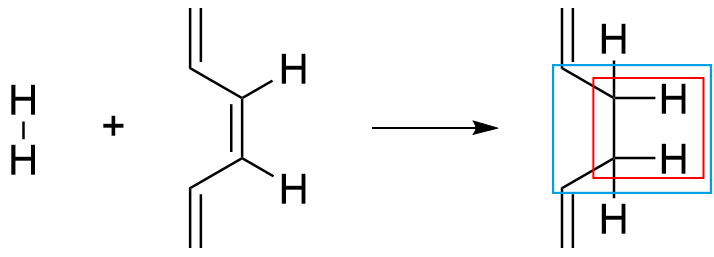
\includegraphics[scale=0.25]{./figures/c6h8.png}
    \caption{这里是图片注释。}
    \label{fig:c6h8} 
    \vspace*{0.35cm}
\end{figure}
图\ref{fig:c6h8}描绘了加成反应的示意图。分子的很大一部分涉及共轭$\pi$键,这对许多量子嵌入方法来说都是比较难以解决的问题。此外,过渡态(定义为势能表面的一阶鞍点)对于一些简单电子结构方法来说也难以描述清楚。
\xmusection{表格}{table}
\begin{table}[!htb]
    \centering
    \caption{这里是表格注释。}
    \label{database}
    \begin{tabular}{ccccc}
        \toprule[1pt]
        \bf\songti 方法/基组 & \bf\songti $E_\text{RS}$ (Hartree) & \bf\songti $E_\text{TS}$ (Hartree) & \bf\songti $\Delta E$ (kcal/mol) & \bf\songti CPU time (s) \\ \midrule[0.75pt]
        ROHF/def2svp & -2831.2668477 & -2831.1564060 & 69.3032 & $1.103 \times 10 ^{5}$ \\ 
        UKS/def2svp & -2840.7439266 & -2840.7098161 & 21.4047 & $1.810 \times 10 ^{5}$ \\ 
        CAS(9o,11e)/def2svp & -2831.3552550 & -2831.3190575 & 22.7140 & $7.938 \times 10 ^{5}$ \\
        DMET(9o,11e)/def2svp & -2831.3520451 & -2831.3156374 & 22.8462 & $1.903 \times 10 ^{5}$ \\ \bottomrule[1pt]
    \end{tabular}
\end{table}


%%%%%%%% 参考文献 %%%%%%%%
\titleformat{\chapter}{\centering\sf\zihao{-3}}{\thechapter}{0.5em}{}
\begin{reference}
    \bibliography{publications.bib}
\end{reference}

%%%%%%%% 致谢(默认在最后) %%%%%%%%

\end{document}
